\documentclass[output=paper,colorlinks,citecolor=brown]{langscibook} 
\author{Heather Bliss\affiliation{Simon Fraser University}\orcid{}\lastand Martina Wiltschko\affiliation{Institució Catalana de Recerca i Estudis Avançats, Universitat Pompeu Fabra}\orcid{}}
\markuptitle{\textit{Stsíkiistsi ki stsíkiistsi}: The ubiquity of Blackfoot demonstratives in discourse}{``Stsíkiistsi ki stsíkiistsi'': The ubiquity of Blackfoot demonstratives in discourse}
\renewcommand{\lsCollectionPaperFooterTitle}{\noexpand\textit{Stsíkiistsi ki stsíkiistsi}: The ubiquity of Blackfoot demonstratives in discourse}

\abstract{Blackfoot demonstratives are ubiquitous and richly polysynthetic, yielding an inventory of 900 unique demonstrative forms. In oral stories, the distribution of demonstratives is particularly broad, and many appear with no clear referent or nominal complement, making no semantic contribution to the propositional content of the utterance. These “untranslatable” demonstratives are the focus of this chapter. Drawing on data from oral stories, we catalogue the properties of untranslatable demonstratives as a means to identify their discourse functions, and we demonstrate that different morphological and prosodic properties encode different discourse functions such as epistemic stance, noteworthiness, and emotivity.}
\IfFileExists{../localcommands.tex}{
  % add all extra packages you need to load to this file

\usepackage{tabularx,multicol}
\usepackage{url}
\urlstyle{same}

\usepackage{listings}
\lstset{basicstyle=\ttfamily,tabsize=2,breaklines=true}

\usepackage{tabularx}
\usepackage{langsci-optional}
\usepackage{langsci-lgr}
\usepackage{langsci-gb4e}

\usepackage[linguistics,edges]{forest}

\usepackage{tikz}





  \newcommand*{\orcid}{}

\makeatletter
\let\thetitle\@title
\let\theauthor\@author
\makeatother

\newcommand{\togglepaper}[1][0]{
  \bibliography{../localbibliography}
  \papernote{\scriptsize\normalfont
    \theauthor.
    \thetitle.
    To appear in:
    Change Volume Editor \& in localcommands.tex
    Change volume title in localcommands.tex
    Berlin: Language Science Press. [preliminary page numbering]
  }
  \pagenumbering{roman}
  \setcounter{chapter}{#1}
  \addtocounter{chapter}{-1}
}

\newcommand{\glopa}{\textsc{opa}}
\newcommand{\glme}{\textsc{top}}
\newcommand{\glte}{\textsc{nfin}}
\newcommand{\glta}{\textsc{nfin}}
\providecommand{\citegen}[1]{\citeauthor{#1}'s (\citeyear*{#1})}

% \newcommand{\sectref}[1]{Section~\ref{#1}} 
  %% hyphenation points for line breaks
%% Normally, automatic hyphenation in LaTeX is very good
%% If a word is mis-hyphenated, add it to this file
%%
%% add information to TeX file before \begin{document} with:
%% %% hyphenation points for line breaks
%% Normally, automatic hyphenation in LaTeX is very good
%% If a word is mis-hyphenated, add it to this file
%%
%% add information to TeX file before \begin{document} with:
%% %% hyphenation points for line breaks
%% Normally, automatic hyphenation in LaTeX is very good
%% If a word is mis-hyphenated, add it to this file
%%
%% add information to TeX file before \begin{document} with:
%% \include{localhyphenation}
\hyphenation{
affri-ca-te
affri-ca-tes
ana-phor-ic
poly-semy
Spra-chen
Fi-scher
Al-chemist
de-mon-stra-tive
Mül-ler
Brea-ker
Hix-kar-ya-na
Que-chua
Unga-rin-jin
Alam-blak
Wam-bon
da-ta-base
quasi-quo-ta-tions
Pisch-lö-ger
de-mon-stra-tions
Ar-khan-gel-skiy
}
\hyphenation{
affri-ca-te
affri-ca-tes
ana-phor-ic
poly-semy
Spra-chen
Fi-scher
Al-chemist
de-mon-stra-tive
Mül-ler
Brea-ker
Hix-kar-ya-na
Que-chua
Unga-rin-jin
Alam-blak
Wam-bon
da-ta-base
quasi-quo-ta-tions
Pisch-lö-ger
de-mon-stra-tions
Ar-khan-gel-skiy
}
\hyphenation{
affri-ca-te
affri-ca-tes
ana-phor-ic
poly-semy
Spra-chen
Fi-scher
Al-chemist
de-mon-stra-tive
Mül-ler
Brea-ker
Hix-kar-ya-na
Que-chua
Unga-rin-jin
Alam-blak
Wam-bon
da-ta-base
quasi-quo-ta-tions
Pisch-lö-ger
de-mon-stra-tions
Ar-khan-gel-skiy
} 
  \togglepaper[1]%%chapternumber
}{}

\begin{document}
\maketitle
\shorttitlerunninghead{The ubiquity of Blackfoot demonstratives in discourse}

%still to be done:
%Tables still to be formatted
%How are URLs displayed in the references? Benus et al. 2007 and Rett 2018 should be given with their URLs

\section{Introduction}\label{sec:bliss:1}

Demonstratives in Blackfoot (ISO 639-3: bla), a Plains Algonquian language spoken in Alberta and Montana, are ubiquitous, fulfilling a wide variety of syntactic functions as determiners, pronouns, predicates, and temporal expressions.\footnote{The title of our paper \textit{Stsíkiistsi ki stsíkiistsi} reflects the ubiquity of deictic elements in Blackfoot more generally. Translating loosely as ‘others and others’, it is comprised of conjoined and pluralised forms of the deictic root \textit{stsíkii}, which has no apparent morphological relationship to other demonstrative or pronominal paradigms.} Demonstratives themselves are polysynthetic in Blackfoot, comprised of up to six morphemes which yields 900 unique forms. In oral stories, the distribution of demonstratives is particularly broad; in addition to their aforementioned uses, they can be used without any clear referent or nominal complement and without any truth-conditional contribution to the content of the utterance. An example of this use of the demonstratives is given in \REF{ex:bliss:1}.\footnote{Data drawn from oral stories are listed with the storyteller’s name (if available) and the title of the story. Uncited examples come from the first author’s field notes. Examples are represented in the Blackfoot orthography developed by \citet{Frantz1978}.} The demonstrative \textit{mii} here does not refer to any discourse referent nor does it have any of the other functions typically associated with demonstratives, as we will show. It seems untranslatable into English. 

\ea\label{ex:bliss:1} (Beatrice Bullshields: \textit{Itohkanao’tsisiyo’p})\\
{Mii ki oostówawáyi stámsaomatapooyaa.}\\
\gll am-yi ki o-isto-wa-ayi stam-sa-omatap-oo-yi-aawa\\
     \textsc{dem-obv} \textsc{conj} \textsc{3-prn-prox-pred} just-out-start-go.\textsc{ai-pl-3pl.prn}\\
     \glt ‘They started out.’
\z

We refer to these demonstratives as “untranslatable” and we propose that these demonstratives function as discourse markers. Drawing on data from a corpus of nearly 100 oral stories, we document which demonstratives can be used in which discourse contexts and we identify the morphological and prosodic properties that encode different discourse functions such as the knowledge states of the interlocutors (\textit{epistemicity}), their emotional states (\textit{emotivity}), as well as how significant the contribution is to the conversation in context (\textit{noteworthiness}). As such, the primary contribution of this chapter is empirical. To our knowledge, this is the first paper that documents the properties of untranslatable demonstratives in Blackfoot, and by mapping morphological and prosodic features onto discourse functions we are laying the foundation for further analysis of Blackfoot demonstratives as discourse markers.

The chapter proceeds as follows. In \sectref{sec:bliss:2}, we outline the sources of our data and our methodology for cataloguing demonstratives. In \sectref{sec:bliss:3}, we describe Blackfoot demonstratives in terms of their morphological composition and syntactic distribution. In \sectref{sec:bliss:4}, we narrow our focus to the untranslatable demonstratives, and we examine the mappings between morphological and prosodic properties and discourse functions. In \sectref{sec:bliss:5}, we provide further evidence for our proposal by showing that particles and demonstratives form a natural class with other units of language that can function as discourse markers. In \sectref{sec:bliss:6}, we conclude.


\section{Sources of data and methodology}\label{sec:bliss:2}

%Integrate URL into footnote
The primary source of data in this chapter is the Blackfoot Oral Stories Database,\footnote{Available at \url{http://stories.blackfoot.atlas-ling.ca}.} an ongoing project developed by the first author in collaboration with members of the Siksika and Kainai communities of Southern Alberta, Canada (see \citealt{BlissEtAl2019}). At the time of writing, the collection consisted of 95 oral stories (comprising approximately 350 minutes of audio recordings) told by 21 storytellers. Not all of the stories are transcribed and not all of them are publicly available on the website. Most of the stories in the collection were curated in group storytelling sessions, in which storytellers gather to share stories with each other, often around a particular theme. Other sources of data include \citegen{RussellGenee2014} collection of eight stories, the Glenbow Museum’s online collection of eight stories,\footnote{Available at \url{https://www.glenbow.org/blackfoot/}.} and the first author’s field notes (2003-2019), which do not contain stories but isolated sentences or short monologues elicited under specific discourse conditions. Unlike the database, all the stories in the two other story collections are fully transcribed,\footnote{A small number of the texts in the database include full or partial morphological analysis, whereas none of those in \citeauthor{RussellGenee2014} collection do. Four of the eight texts in the Glenbow collection have been analysed and glossed by the first author of this chapter.} and our understanding is that these stories were recorded in more formal settings (i.e. a single speaker alone in a sound booth). Data from field notes is not analysed in terms of discourse properties but is used in this chapter to provide background information on the grammar of demonstratives and particles.

There are two limitations to using this corpus for investigating the discourse properties of demonstratives. First, because it consists entirely of monologic texts, the corpus includes no conversation data, which presumably would be the most fertile environment for observing discourse functions. However, as noted, many of the stories in the database were curated in group settings which tend to be rather informal and conversational in nature, and these show a marked difference from those curated in more formal contexts. We discuss this in more detail in \sectref{sec:bliss:4.5} below. Second, stories from the \citet{RussellGenee2014} collection and the Glenbow collection are available as transcripts rather than audio recordings, and as such it is impossible to know whether there are any omissions from these transcripts that are relevant to this study, namely untranslatable material such as demonstratives.

Limitations aside, the corpus contains approximately 5100 demonstratives, which were catalogued according to their morphological, prosodic,\footnote{In terms of prosodic properties, we catalogued vowel lengthening and reduplication. Pitch accent is also marked on the demonstratives but is yet to be catalogued and analysed. See \sectref{sec:bliss:3.1} for discussion.} distributional, and discourse properties. For un-transcribed audio recordings, translation assistance was provided by Siksika Elder and fluent speaker Ikino’motstaan Noreen Breaker. For the purpose of analysing untranslatable demonstratives, all demonstrative tokens with an obvious referent or nominal complement, and/or a clear semantic contribution to the propositional content of the utterance were set aside. All demonstratives with a “verbalising” suffix suggestive of a predicative function were also set aside. The remaining 530 forms comprise the corpus of untranslatable demonstratives; these were analysed for correlations between morphological/prosodic properties and discourse functions. These correlations are discussed in \sectref{sec:bliss:4}, following a brief introduction to the composition and distribution of demonstratives more broadly. 


\section{Blackfoot demonstratives: An overview}\label{sec:bliss:3}

\subsection{Composition of demonstratives}\label{sec:bliss:3.1}

Demonstratives in Blackfoot are morphologically complex, comprised of an obligatory demonstrative root plus up to five optional suffixes, as illustrated in \figref{fig:bliss:1} (descriptions of the roots and inflections are given in \sectref{sec:bliss:4} below; see also \citet{Bliss2013}, \citet{Frantz2017}, \citet{Schupbach2013} for detailed descriptions of the other morphemes, which are not of central importance to this chapter). There are no combinatoric restrictions on the composition of demonstratives, meaning that there are 900 possible demonstrative forms.

  
\begin{figure}
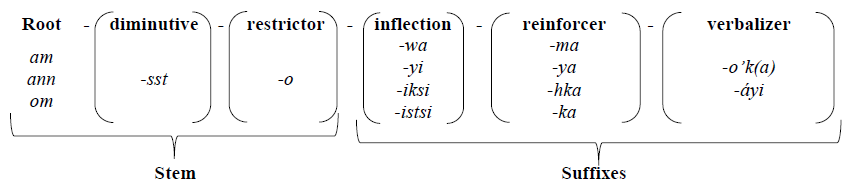
\includegraphics[width=\textwidth]{figures/6_Figure1.png}
\caption{Blackfoot demonstrative template}
\label{fig:bliss:1} 
\end{figure}

In addition to these 900 forms, demonstratives can show variation based on prosodic properties, as described below. 

Blackfoot is a pitch accent language (see, e.g., \citealt{VanDerMark2003}), and accent can be variably assigned to different syllables on the demonstratives. The semantic and/or pragmatic contributions of pitch accent on the demonstratives are not yet well understood, but \citet{Schupbach2013} observes correlations with syntactic function (i.e. different pitch accent patterns based on whether demonstratives function as a determiners or pronouns) and speculates that there may also be specific pitch accent patterns for topicalised demonstratives. An analysis of the pitch accent patterns for the untranslatable demonstratives is pending, and as such pitch accent is not further discussed in this chapter.

Vowel lengthening and reduplication are also attested for demonstratives, the latter in particular with the untranslatable ones. These are discussed in \sectref{sec:bliss:4.4} Finally, demonstratives are often combined with particles, particularly the conjunction particle \textit{ki}. Particles are discussed in \sectref{sec:bliss:5}


\subsection{Distribution of demonstratives}\label{sec:bliss:3.2}

Like demonstratives in many other languages, demonstratives in Blackfoot can function as either determiners or pronouns, but they also have a broader distribution, as will be observed throughout this section and in \sectref{sec:bliss:4} below. Regarding their distribution as determiners, they are the only determiner-like elements in Blackfoot, and they have a canonical determiner-like distribution. They are required with arguments, as shown in \REF{ex:bliss:2} and ungrammatical with predicate nominals (which we assume are pseudo-incorporated, see \citealt{Bliss2018}), as shown in \REF{ex:bliss:3}.

\ea\label{ex:bliss:2} {Kikatao’tsiksiiststoo’paatsiks *(omistsi) pisátssaisskiists?}\\
\gll kit-kata’-otsiksiiststoo-’p-wa-atsiks om-istsi pisatssaisski-istsi\\
     2-\textsc{interr}-water.\textsc{ti-1:inan-prox-3sg.prn} \textsc{dem-pl} flower-\textsc{pl}\\
\glt ‘Did you water the flowers?’
\z

\ea\label{ex:bliss:3} {Nitáíkskimaa (*oma) ponoká.}\\
\gll nit-a-ikskimaa ponoka\\
     1-\textsc{impf}-hunt.\textsc{ai} elk\\
\glt ‘I am elk-hunting.’
\z

In \REF{ex:bliss:2}, the demonstrative \textit{omistsi} cannot be omitted (as indicated by the asterisk outside the brackets, and in \REF{ex:bliss:3}, the demonstrative \textit{oma} cannot be included (as indicated by the asterisk inside the brackets). As pronouns, demonstratives can be interpreted as human or non-human, definite or indefinite, as shown in \REF{ex:bliss:4} through \REF{ex:bliss:6}.

\ea\label{ex:bliss:4} {Nimáátowaanihpa ann.}\\
\gll nit-matt-waanii-hpa ann\\
    1-\textsc{neg}-say.\textsc{ai-nonaff} \textsc{dem}\\
\glt ‘I am not saying that.’
\z

\ea\label{ex:bliss:5} {Annoma ita’páíssiwa.}\\
\gll ann-o-ma it’ap-a-issi-wa\\
    \textsc{dem-restr-stat} \textsc{loc}-around-\textsc{impf}-be.\textsc{ai-prox}\\
\glt ‘She’s around here.’
\z

\ea\label{ex:bliss:6} (Lena Russell: \textit{Ksissta’pssiwa}) \\
{Ísstsiiwoka ámohka awaasáíí’niwahka.}\\
\gll yisstsii-k-wa am-o-hka a-waasaii’ni-wa-hka\\
  listen-\textsc{imp.pl-prox} \textsc{dem-restr-invis} \textsc{impf}-cry.\textsc{ai-prox-rep}\\
\glt ‘Listen to someone crying.’ 
\z

In addition to functioning as determiners and pronouns, demonstratives can function as predicates. In this usage, they typically (but not necessarily) appear with a “verbalising” suffix, as shown in \REF{ex:bliss:7} and \REF{ex:bliss:8}.

\ea\label{ex:bliss:7} {Óómahko’ka.}\\
\gll oom-wa-hk-o’ka\\
     \textsc{dem-prox-invis-vbzr}\\
\glt ‘It’s way over there.’
\z

\ea\label{ex:bliss:8} (Glenbow: \textit{Miohpokoiksi})\\
{Annimai akitaahsaopiiyaawa.}\\
\gll ann-yi-ma-ayi yaak-it-aahsa-opii-yi-aawa\\
     \textsc{dem-obv-stat-vbzr} \textsc{fut-loc}-always-stay.\textsc{ai-pl-3pl.prn}\\
\glt ‘And that is where they will always stay.’ 
\z

Demonstratives can also be interpreted as temporal expressions in Blackfoot. Temporal demonstratives can have any of the syntactic functions described above: they can be determiners, pronouns, or predicates. Demonstratives are often (but not always) clause-initial when they receive a temporal interpretation, and they often (but not always) are marked with the “other time” suffix -\textit{ka}, as in \REF{ex:bliss:9} and \REF{ex:bliss:10}.

\ea\label{ex:bliss:9} (Beatrice Bullshields: \textit{Itáísapssiisskiitso’pa})\\ 
{Amoka iisskóóhtsik nitsitsí’nakstssi’pi.}\\
\gll am-o-ka isskoohtsik nit-it-i’naksstssi-hp-yi\\
     \textsc{dem-restr-oth.tm} long.ago 1-\textsc{loc}-be.young.\textsc{ai-conj.nom-obv}\\
\glt ‘Long ago when I was young.’ 
\z

\ea\label{ex:bliss:10} (Glenbow: \textit{Katoyissa})\\
{Katoyissa anohk iitayo’kayihk omistsi Katoyissiksi.}\\
\gll Katoyissa ann-o-hk ii-it-a-yo’kaa-ihk om-istsi Katoyissiksi\\
     K. \textsc{dem-restr-invis} \textsc{ic-loc-impf-}sleep\textsc{.ai-rep} \textsc{dem-pl} Sweet.Pine.Hills\\
\glt ‘Katoyissa now sleeps at Sweet Pine Hills.’ 
\z

%Reconsider last sentence in this paragraph
In addition to their determiner, pronoun, predicate, and temporal uses, demonstratives are found with an even broader distribution in discourse contexts, particularly oral stories that are told in a conversation-like setting. These demonstratives do not have a clear referent or nominal complement, they do not contribute to the truth-conditional content of the utterance, and as such they cannot (easily) be translated. An example was given in \REF{ex:bliss:1}, and a second example is given in \REF{ex:bliss:11}. 

\ea\label{ex:bliss:11} (Beatrice Bullshields: \textit{Itáísapssiisskiitso’pa})\\
{Anna nóóhkohpoksapopiimook anna Tóótsinam.}\\
\gll ann-wa noohk-ohpok-sapopii-m-ok ann-wa Tóótsinam\\
     \textsc{dem-prox} please-\textsc{accomp}-ride\textsc{-ta-accomp-2pl:3.imp} \textsc{dem-prox} T.\\
\glt ‘Please ride with Tootsinam!’ 
\z

The first instance of the demonstrative \textit{anna} in \REF{ex:bliss:11} does not refer to an individual and it cannot be interpreted as either a predicate or temporal expression. Nor does it introduce a nominal complement; the second but not the first instance of \textit{anna} functions as a determiner for the proper noun \textit{Tóótsinam} (proper nouns in Blackfoot are often used with demonstrative determiners, see \citet{Bliss2013} for examples and discussion). In short, the first instance of \textit{anna} cannot be analysed as a determiner, pronoun, predicate, or temporal expression. Demonstratives of this variety are frequently found in oral stories, often clause-initially, and we refer to them as “untranslatable”. We discuss their properties at length in \sectref{sec:bliss:4}. 

\section{“Untranslatable” demonstratives}\label{sec:bliss:4}

\subsection{Overview}\label{sec:bliss:4.1}

In this section, we focus exclusively on the untranslatable demonstratives. As observed in \sectref{sec:bliss:3.1}, demonstratives vary along numerous morphological and prosodic dimensions. Here we look at which demonstratives are attested as untranslatable, and what the variation in untranslatable demonstratives can tell us about their discourse properties. We observe that a wide range of untranslatable demonstrative forms are attested, and that their morphological and prosodic variation correlates with properties typically associated with discourse markers, such as epistemicity, noteworthiness, and emotivity. 

\subsection{Demonstrative roots}\label{sec:bliss:4.2}

When they function as determiners or pronouns, demonstratives are built from one of three roots, which are categorised according to a person-based proximity system, shown in \tabref{tab:bliss:1}.

%Adjust table width
\begin{table}
\begin{tabularx}{\textwidth}{Xl}
\lsptoprule
\textbf{Form} & \textbf{Meaning}\\
\midrule
\textit{am-} & Proximity to speaker\\
\textit{ann-} & Proximity to addressee\\
\textit{om-} & Proximity to neither speaker nor addressee\\
\lspbottomrule
\end{tabularx}
\caption{Demonstrative roots}
\label{tab:bliss:1}
\end{table}

All three of these roots are attested with untranslatable demonstratives\footnote{The initial vowel of untranslatable and other demonstratives is frequently dropped, obscuring the distinction between the \textit{am}- and \textit{om}- forms. In our corpus of untranslatable demonstratives, there are only three \textit{om}- forms (with the initial vowel retained) and no \textit{am}- ones. We assume that all of the \textit{m}- forms are underlyingly \textit{am}- based on their distribution.} but they appear in different discourse contexts. All of the \textit{am}- and \textit{ann}-forms appear in complementary distribution, with \textit{am}- being used when the content of the proposition is something expected, predictable, or familiar to the addressee \REF{ex:bliss:12}, and \textit{ann}- being used when the content of the proposition is something unexpected, surprising, or new to the addressee \REF{ex:bliss:13}.

\ea\label{ex:bliss:12} (Clifford Crane Bear: \textit{Who’s in Charge?})\\
{Miiii náó’tapssapiwa otááksikamotaa’si.}\\
\gll am-yi na-o’tap-ssapi-wa ot-yaak-ikamotaa-hs-yi\\
     \textsc{dem-obv} \textsc{evid}-return-look.\textsc{ai-prox} \textsc{3-fut}-give.birth.\textsc{ai-conj-obv}\\
\glt [A grandfather is trying to find someone who can transport his labouring wife to the hospital. After a few unsuccessful attempts, he returns home to check on his wife and then:] ‘He returned to seeking help for her to give birth.’ 
\z

\ea\label{ex:bliss:13} (Mildred Three Suns: \textit{Appapaainihkssin})\\
{Kiann nitáíto’too itohkanáópiiyaa itáákopiyaa áíkaahsiyaa.}\\
\gll ki-ann nit-a-it-o’too it-ohkana-opii-yaawa it-yaak-opii-yaawa a-ikaahtsi-yi-aawa\\
     \textsc{conj-dem} \textsc{1-impf-loc}-arrive.\textsc{ai} \textsc{loc-}all-sit-\textsc{3pl} \textsc{loc-fut}-sit-\textsc{3pl} \textsc{impf}-gamble-\textsc{3pl-3pl.prn}\\
\glt [(Describing a dream:) The speaker hears music and is wandering around, trying to locate its source. Finally:] ‘I arrived there and these people were all sitting, they would just sit there gambling.’ 
\z

In \REF{ex:bliss:12}, the demonstrative \textit{miiii} is used in a sentence that reports a repeated event in the context of the narrative, namely the grandfather returning home yet again. As a repeated event, it is something that the audience (/addressee) could predict in the context of the narrative. Other instances of untranslatable demonstratives formed from the \textit{am}- root have a similar distribution in narratives; they are used when the information is familiar or expected, often because it refers to repeated events in the story. Conversely, in \REF{ex:bliss:13} the demonstrative \textit{kiann} is used at a point in the narrative when the speaker is recounting her discovery of something new and unexpected; it is surprising. In other narratives, untranslatable demonstratives formed from the \textit{ann}- root are used with a similar distribution. 

While the fact that the untranslatable demonstratives can function as markers of epistemicity status is not really surprising, the particular way in which they do this in Blackfoot is. The marking of epistemicity can be understood if we observe the fact that demonstratives are often used to mark the discourse status of referents. For example, in English (as in many other languages) demonstratives can be used to mark spatial deixis indicating whether the referent is close or far from the deictic centre (\textit{this} vs. \textit{that}). However, spatial deixis is not the only dimension of contrast. Other common uses of demonstratives include anaphoric, discourse deictic, and recognitional uses (see \citet{Diessel1999Book} for an extensive crosslinguistic overview). Of particular interest to us is the discourse deictic use, which refers to the use of demonstratives as referring to propositions. This means that the demonstratives cannot only refer to individuals, but also to propositions. This is akin to the use of Blackfoot demonstratives under consideration here: they don’t refer to individuals but instead they are used to express the epistemic state of the interlocutor relative to the proposition that hosts them. 

Moreover, the recognitional use of demonstratives is also relevant: it refers to the use of demonstratives as indicating whether the referent is novel or familiar to the speaker, as in the English examples in \REF{ex:bliss:14}. With the use of \textit{this} in \REF{ex:bliss:14a}, the speaker indicates that the referent is novel to the addressee; it is not part of the common ground. In contrast, in \REF{ex:bliss:14b} the use of \textit{that} indicates that the speaker assumes that the addressee is familiar with the referent; it is part of the common ground. 

\ea\label{ex:bliss:14}
\ea\label{ex:bliss:14a} A few years ago I saw this movie with Klaus Kinski.\\
\ex\label{ex:bliss:14b} Do you remember that movie we saw with Klaus Kinski?\\
\z
\z

\citet{ColasantiWiltschko2019} demonstrate that this pattern is not restricted to English, but instead is found in many genetically and geographically unrelated languages, including Italian, German, Japanese, Medumba, Spanish, French, Southern Italo-Romance, and Cantonese. 

Thus, for the Blackfoot demonstratives to indicate whether a given proposition is expected (/familiar) or unexpected (/novel) falls within this general use of demonstratives. However, there is one caveat: the Blackfoot pattern seems to be the exact opposite of what is observed in English and other languages. The root \textit{am}, which can be used to indicate closeness to the speaker, would appear to be the equivalent to proximate demonstratives. But unlike proximate demonstratives in other languages, Blackfoot \textit{am} indicates familiarity. 

This unexpected pattern requires further research. In particular, it is necessary to carefully explore the use of the untranslatable demonstratives in conversations. Storytelling is a different kind of genre, where the interlocutors play different roles. For now, we speculate that a potential key to this conundrum might lie in the temporal use of Blackfoot demonstratives. In particular, recall from \REF{ex:bliss:9} and \REF{ex:bliss:10} that \textit{am} is used to indicate temporal distance, whereas \textit{ann} is used to indicate temporal proximity. 

In sum, we have now seen that the untranslatable demonstratives can be used to mark the epistemic states of the interlocutors relative to the proposition. In this respect they carry a similar functional load to discourse markers in other languages (see \citealt{Ariel1998}; \citealt{Schiffrin1987}), including so-called “discourse particles” in German (\citealt{Thoma2017}; \citealt{Zimmermann2011}) and Cantonese \citep{Lam2014}, as well as discourse markers and enclitics in related Algonquian languages such as Ojibwe \citep{Fairbanks2016} and Meskwaki \citep{Goddard2015}.

Following the hypothesis that the demonstrative roots encode epistemicity, we predict that the \textit{om}- forms should also pattern together with respect to epistemic orientation, but this is not the case. The caveat, however, is that there are only three examples with \textit{om}- and it is hard to draw reliable conclusions from such a small data set. 

\subsection{Demonstrative inflection}\label{sec:bliss:4.3}

When they function as determiners or pronouns, demonstratives can take the same inflection as nouns. Blackfoot nominal inflection encodes number, animacy, and obviation distinctions, as shown in \tabref{tab:bliss:2}.

%adjust column width
\begin{table}
\begin{tabularx}{.8\textwidth}{XXXl}
\lsptoprule
&  & \textbf{Animate} & \textbf{Inanimate}\\
\midrule
\textbf{Singular} & \textbf{Proximate} & \textit{-wa} & \textit{-yi}\\
\textbf{Singular} & \textbf{Obviative} & \textit{-yi} & \textit{-yi}\\
\textbf{Plural} & {} & \textit{-iksi} & \textit{-istsi}\\
\lspbottomrule
\end{tabularx}
\caption{Demonstrative inflection}
\label{tab:bliss:2}
\end{table}

Whereas number inflection is relatively straightforward, animacy and obviation require brief explanations. Regarding animacy, all nouns in Blackfoot (and other Algonquian languages) are inherently categorised as animate or inanimate, but this grammatical designation does not always straightforwardly map onto ontological distinctions of animacy (i.e. not all animate nouns refer to what we tend to think of as animate individuals, at least under a Eurocentric worldview).\footnote{Some authors have suggested that Algonquian animacy distinctions may be motivated by ontological properties more congruent with an Indigenous worldview (such as “power potential”), suggesting that “animacy” is perhaps the wrong label for this category (see, e.g., \citealt{Dahlstrom1995}, \citealt{Goddard2002}).} Obviation is a reference-tracking device common to Algonquian languages; the more salient participant in a stretch of discourse is marked proximate and all subsidiary participants are marked obviative (see, e.g., \citealt{Bliss2017Dependencies}; \citealt{Dahlstrom1991}; \citealt{Genee2009}; \citealt{Goddard1984}, \citeyear{Goddard1990}; \citealt{Junker2004}). Obviation is typically restricted to third persons in Algonquian languages, although first and second person independent pronouns are also marked with proximate and obviative inflection in Blackfoot. As observed in \tabref{tab:bliss:2}, the proximate-obviative contrast is neutralised with inanimate and plural third persons; the syncretism between animate obviative and inanimate proximate/obviative can be considered accidental (see \citealt{BlissOxford2016}, \citeyear{BlissOxford2017}). Demonstrative determiners usually take the same inflection as the nouns they modify, with some exceptions (see \citealt{Bliss2017Demonstratives} on demonstrative-noun mismatches).

Whereas the full range of nominal inflection is attested when the demonstratives function as pronouns or determiners, only -\textit{wa} (proximate singular) and -\textit{yi} (obviative singular) are attested with the untranslatable demonstratives. Just as these inflections encode relative saliency when they appear on nouns and pronouns, they also appear to encode relative saliency when they appear on the untranslatable demonstratives. All of the proximate-marked demonstratives appear in sentences that coincide with salient or noteworthy events in the story (corresponding with, for example, plot twists or important points in the arc of the narrative), whereas all of the obviative-marked demonstratives appear elsewhere, without this same sense of noteworthiness. As such, the obviative-marked demonstratives are much more frequent, seemingly used as a default inflection. Representative examples of proximate and obviative forms are given in \REF{ex:bliss:15}-\REF{ex:bliss:16}.

\ea\label{ex:bliss:15} (Beatrice Bullshields: \textit{Sa’aiwa)}\\
{Kimaa ki ama nitómitaaminnaan mattsistáó’hkoonima omi oyííyiskaassini.}\\
\gll ki-am-wa ki am-wa nit-omitaa-m-innaan mattsista’-ohkooni-m-wa om-yi oyiiyis-kaa-ssin-yi\\
     \textsc{conj-dem-prox} \textsc{conj} \textsc{dem-prox} \textsc{1-}dog-\textsc{poss-1pl} again-find.\textsc{ti-3:inan-prox} \textsc{dem-inan} nest-?-\textsc{nom-inan}\\
\glt [A child is trying to protect some unhatched duck eggs, but the family dog repeatedly finds the nest and eats the eggs. This is the third and final time the dog does this before the child makes a drastic move to protect the one remaining egg:] ‘And then our dog found the nest again.’ 
\z

\ea\label{ex:bliss:16} (Clifford Crane Bear: \textit{Isttstsáápikimmiksi})\\
{Kiannika isáma’piiwa.}\\
\gll ki-ann-yi-ka isam-a’pii-wa\\
     \textsc{conj-dem-obv-oth.tm} long.time-be.\textsc{ii-prox}\\
\glt [A grandfather is being questioned by the police and, as an aside, the storyteller notes that he had to wait for his grandfather to return:] ‘It was a long time.’ 
\z

The demonstrative \textit{kimaa} in \REF{ex:bliss:15} is formed from the root \textit{am}- which, as we saw in the preceding section, functions to mark the utterance as containing familiar or expected information. In this example, as with many others, the information is expected because it is a repeated event in the narrative. However, although expected information, it is nevertheless noteworthy: this is a pinnacle point in the story which results in a major plot twist. The proximate marking -\textit{wa} on the demonstrative foregrounds the event and signals to the audience that it is noteworthy or salient in the story. Conversely, the demonstrative \textit{kiannika} in \REF{ex:bliss:16} is marked with the obviative suffix -\textit{yi}, and the event denoted by the utterance is not one of particular significance in the story; it is simply an aside to the main event of the grandfather being held captive. 

The function of noteworthiness is attested for discourse markers in other languages as well. For example, \citet{Jónsson2017} notes that the Icelandic particles \textit{en}, \textit{vá}, and \textit{œ} are required by some speakers with certain exclamatives to give them their noteworthy flavour. 

\subsection{Other demonstrative properties}\label{sec:bliss:4.4}

The preceding sections looked at two sources of morphological variation in the demonstratives: root distinctions and inflectional distinctions. As observed in \figref{fig:bliss:1}, demonstratives exhibit other morphological variation as well. In addition to the inflectional suffixes, there are four other suffixes that can be added to the demonstrative roots. While some of these suffixes are attested with untranslatable demonstratives (see, e.g., \REF{ex:bliss:16} for the ‘other time’ suffix -\textit{ka}), there are no detectable patterns of distribution in the corpus that would suggest these suffixes encode discourse functions. 

However, vowel lengthening does appear to serve a discourse function with the untranslatable demonstratives. When the demonstratives are used deictically (i.e. as pronouns or determiners), vowel lengthening is iconic: the further away the referent is from the speaker, the longer the vowel is \REF{ex:bliss:17}.

\ea\label{ex:bliss:17}
\ea No lengthening\\
  Na Carmelle íínoyiiwa omi ksisskstakii.\\
\gll  ann-wa Carmelle ii-in-o-yii-wa om-yi ksisskstaki-yi \\
     \textsc{dem-prox} C. \textsc{ic}-see-\textsc{ta-dir-prox} \textsc{dem-obv} beaver-\textsc{obv}\\
\glt ‘Carmelle saw that beaver (nearby).’

\ex Slight lengthening\\
  Na Carmelle íínoyiiwa oomi ksisskstakii.\\
\gll  ann-wa Carmelle ii-in-o-yii-wa om-yi ksisskstaki-yi  \\
     \textsc{dem-prox} C. \textsc{ic}-see-\textsc{ta-dir-prox} \textsc{dem-obv} beaver-\textsc{obv}\\
\glt ‘Carmelle saw that beaver (way over there).’

\ex Pronounced lengthening\\
  Na Carmelle íínoyiiwa ooomi ksisskstakii.\\
\gll  ann-wa Carmelle ii-in-o-yii-wa om-yi ksisskstaki-yi  \\
     \textsc{dem-prox} C. \textsc{ic}-see-\textsc{ta-dir-prox} \textsc{dem-obv} beaver-\textsc{obv}\\
\glt ‘Carmelle saw that beaver (waaaayyy over there).’
\z
\z

Vowel lengthening is also found with the untranslatable demonstratives and is sometimes quite pronounced, as in \REF{ex:bliss:18}. In this example, the vowel of the demonstrative is extra-long with a duration of 0.877 seconds (compare this duration with that of the un-lengthened vowel of the conjunction particle \textit{ki}, which is much shorter at 0.073 seconds).

\ea\label{ex:bliss:18} (Clifford Crane Bear: \textit{Isttstsáápikimmiksi})\\
{Kimiiii nitáítopokská’sspiinaan.}\\
\gll ki-am-yi nit-a-itap-okska’si-hpinnaan\\
     \textsc{conj-dem-obv} \textsc{impf-}toward-run\textsc{.ai-1pl}\\
\glt [A young man is helping his grandfather with a task that the police later take notice of; he is confused about why they are doing what they are doing.] ‘And we ran towards (something).’ 
\z

What is the function of vowel lengthening when it appears on the untranslatable demonstratives? Our hypothesis is that vowel lengthening encodes emotivity, i.e. the speaker’s emotive attitude or personal reaction – positive or negative – towards the content of the utterance. In all cases in which the vowel of an untranslatable demonstrative is lengthened, the context is one of heightened emotion within the narrative; consider \REF{ex:bliss:19} and \REF{ex:bliss:20}.

\ea\label{ex:bliss:19} (Beatrice Bullshields: \textit{Itáísapssiisskiitso’pa})\\
{Kimiii nitóhtsitsinnohpii nitsínnoo’takohpi.}\\
\gll ki-am-yi nit-oht-it-inn-ohpi’yi nit-inn-o’tak-ohpi’yi\\
     \textsc{conj-dem-obv} \textsc{1-}means-\textsc{loc-}down-fall.\textsc{ai} \textsc{1}-down-in.circle-fall.\textsc{ai}\\
\glt [A child wants to go sledding with her sisters but they won’t share their sleds. She finds a wash basin and gleefully slides down the snowy hill in the basin.] ‘And with it, I went down, spinning in circles.’ 
\z

\ea\label{ex:bliss:20} (Beatrice Bullshields: \textit{Itohkanao’tsisiyo’p})\\
{Kimiii níísto nisstónnatsotamasapaasai’ni.}\\
\gll ki-am-yi n-iisto nit-sstonnat-sotam-sap-waasai’ni\\
     \textsc{conj-dem-obv} \textsc{1-prn} \textsc{1-}extremely-genuinely-?-cry\textsc{.ai}\\
\glt [A child wants to accompany her grandparents to a ceremonial event, but they tell her she is too young and leave without her.] ‘I kept crying and crying after them.’ 
\z

Both of these examples represent points in their respective stories in which the speaker has a strong emotional connection to the content of the utterance; in \REF{ex:bliss:19} this connection is positive and in \REF{ex:bliss:20} it is negative.

Emotivity is a discourse function encoded by discourse markers in other languages (see, e.g., \citet{Rett2018} on emotive markers like English \textit{alas}), and it has been observed to be achieved via prosodic features such as lengthening and pitch accent (see, e.g., \citet{BenusGravanoHirschberg2007} on English \textit{whatever}). Blackfoot exhibits a similar pattern: vowel lengthening on the untranslatable demonstratives correlates with instances of high emotion. As for \REF{ex:bliss:18}, we suggest that the emotional connection is not with the speaker but with the speaker’s assumptions about the addressee; the storyteller is using vowel lengthening as a means to evoke suspense. All other examples in the corpus with vowel lengthening similarly coincide with strong emotions, either on behalf of the speaker or the addressee.

Whereas vowel lengthening is relatively common on demonstratives regardless of their syntactic function, demonstrative reduplication seems to be restricted to the untranslatable demonstratives only. Moreover, it is used frequently by one particular storyteller (Allan Stevens), less often by another (Mildred Three Suns), and not at all by the remaining 19 storytellers. Based on its limited distribution in the current corpus, it is not possible to ascertain the function of demonstrative reduplication, but we speculate that it may be used for emphatic purposes \REF{ex:bliss:21}.

\ea\label{ex:bliss:21} (Allan Stevens: \textit{O’kaan})\\
{Síksinnaki omi omi máátaanistsi’tooyi miksi matapíksi.}\\
\gll siksinnaki-wa om-yi om-yi maat-waanistsi’to-yii-wa om-iksi matapi-iksi\\
     police-\textsc{prox} \textsc{dem-obv} \textsc{dem-obv} \textsc{neg}-obey.\textsc{ta-dir-prox} \textsc{dem-pl} person-\textsc{pl}\\
\glt [At a Sundance ceremony, a police officer violated ceremonial protocol by crossing in front of some dancers, and later that day he fatalistically broke his leg. The moral of the story:] ‘The policeman didn’t listen to the people.’ 
\z

In \REF{ex:bliss:21}, the storyteller is concluding the story by emphasising the significance of the event and its consequences; this emphasis is encoded by the reduplication of the demonstrative.

\subsection{Summary}\label{sec:bliss:4.5}

In this section we have examined the composition and distribution of untranslatable demonstratives in Blackfoot, mapping their morphological and prosodic properties onto discourse functions. A summary of our hypotheses is presented in \tabref{tab:bliss:3}.

%Adjust column width
\begin{table}
\begin{tabularx}{\textwidth}{lQ}
\lsptoprule
\textbf{Pragmatic function} & \textbf{Demonstrative distinction}\\
\midrule
Epistemicity & Root distinctions\\
Noteworthiness & Inflectional distinctions (proximate/obviative)\\
Emotivity & Vowel lengthening\\
Emphasis (?) & Reduplication\\
\lspbottomrule
\end{tabularx}
\caption{Mapping demonstrative distinctions to pragmatic functions}
\label{tab:bliss:3}
\end{table}

\tabref{tab:bliss:3} shows that demonstratives in Blackfoot can encode a range of discourse functions that are typically associated with discourse markers in other languages. As such, we propose that Blackfoot demonstratives are multi-functional: they can fulfil canonical deictic functions as determiners or pronouns, but they can also fulfil discourse functions that extend beyond the truth-conditional content of the utterance. Given that untranslatable demonstratives are built using the same morphological and prosodic ingredients as all other demonstratives, we suggest that untranslatable demonstratives are not unique lexical items, homophonous with other demonstrative forms, but rather that all demonstratives have the capacity to function in various ways, including as discourse markers. In other words, demonstratives have the capacity to scope over individuals (as pronouns or determiners), times (as temporal expressions), situations (as predicates), or propositions (as discourse markers).

One outstanding question is whether the stories that serve as the data source here truly comprise a set of discourse contexts that are amenable to the use of discourse markers. As noted in \sectref{sec:bliss:2}, most of the stories in the database were curated in group storytelling sessions, which tend to be conversational in nature. To elaborate, in these group sessions, storytellers take turns sharing stories around a particular theme, and while the resulting recordings are indeed monological rather than dialogical, the overarching context is much more like a dialogue or conversation with interlocutors exchanging information by sharing stories with each other. Importantly, it is only in texts from these conversation-like contexts that untranslatable demonstratives are found. More formal settings do not elicit untranslatable demonstratives, as evidenced by the fact that there are no examples of untranslatable demonstratives in the \citet{RussellGenee2014} collection or the Glenbow collection. 

The properties of untranslatable demonstratives just reviewed suggest that they function in similar ways to discourse markers in other languages; they don’t contribute to the propositional content of an utterance but instead serve to manage the ongoing conversation (e.g. \citealt{Ariel1998}; \citealt{Fairbanks2016}; \citealt{Schiffrin1987}). In the following section we discuss further parallels between the untranslatable demonstratives and discourse markers.


\section{Untranslatable demonstratives as discourse markers}\label{sec:bliss:5}


Discourse markers are sometimes dedicated units of language (such as English \textit{eh} and \textit{huh}) and sometimes they are units of language that serve “double duty”: to express propositional content and to express discourse related functions (such as English \textit{right,} \textit{so} and \textit{well}). However, what many discourse markers have in common is that they are often simplex forms which cannot be inflected. As such they are commonly labelled as “particles” (\citealt{Abraham1991}; \citealt{Aijmer2002}; \citealt{Zimmermann2011}). While particles share certain formal properties (they are not complex, they don’t inflect), they are generally not definable in positive terms and hence are not a natural class within and across languages. Nevertheless, it is perhaps not coincidental that discourse markers share these properties across different languages. Hence, in this section, we explore the properties of untranslatable demonstratives from the point of view of discourse markers.

By means of exploring the inventory of particles in Blackfoot, we show that particles that function as discourse markers are relatively rare in the language. At the same time, we show that they form a natural class with demonstratives. This lends further support to our claim that demonstratives in Blackfoot function as discourse markers. 

The Blackfoot Dictionary (\citealt{FrantzRussell1995})\footnote{There is a newer edition of the dictionary (\citealt{FrantzRussell2017}) but we have yet to conduct a search of this dictionary for UND forms.}  lists only 31 entries that are classified as UND (“underived particle”), excluding vocative pronouns and kin terms. These are listed in \REF{ex:bliss:22}.

\ea\label{ex:bliss:22} {Blackfoot underived particles}\\
\ea \textit{saa} ‘no’\\
\ex \textit{áa} ‘yes’\\
\ex \textit{oki} ‘hello’\\
\ex \textit{ki} ‘and’\\
\ex \textit{tsimá} ‘where?’\\
\ex \textit{tsa} ‘how?’ (often used in question formation)\\
\ex \textit{yáóo} \textit{{\textasciitilde} yáa} ‘oh no!’\\
\ex \textit{ha’} ‘pfft! ha!’ (used to express scorn)\\
\z
\z

What these forms have in common is that they are underived particles and many of them function as discourse markers, i.e. they serve to regulate conversational interaction.  

Some of the UND forms listed in the dictionary are concatenations of particles; see, e.g., \REF{ex:bliss:23}.

\ea\label{ex:bliss:23} {Concatenated particle}\\
ha’yaa\\
\gll ha’-yaa\\
     scorn-oh.no\\
\glt ‘uh-oh!’ (in anticipation of a reprimand)
\z

Beyond these underived and concatenated particles, the majority of entries that are classified as UND in the dictionary involve demonstrative morphology in one of three ways. First, some inflected demonstratives are listed in the dictionary as UND forms, as in  \REF{ex:bliss:24} and \REF{ex:bliss:25}. 

\ea\label{ex:bliss:24} {Inflected demonstrative listed as UND in \citet{FrantzRussell1995}}\\
annóhk\\
\gll ann-o-hk\\
     \textsc{dem-restr-invis}\\
\glt ‘right now’
\z

\ea\label{ex:bliss:25} {Inflected demonstrative listed as UND in \citet{FrantzRussell1995}}\\
ánniayi\\
\gll ann-yi-ayi\\
     \textsc{dem-inan-vbzr}\\
\glt ‘that’s enough’
\z

\citegen{FrantzRussell1995} treatment of inflected demonstratives as underived particles suggests they are assuming them to be independent but homophonic lexemes. This differs from the analysis developed here under which inflected demonstratives are multifunctional and can take on a role as discourse markers. Our analysis is supported by the co-variation observed in \sectref{sec:bliss:4} between the morphological and prosodic composition of demonstratives and their various discourse functions.

The preceding example shows one of the three ways in which entries classified as UND in the dictionary involve demonstrative morphology. The second way is one we have seen in earlier examples in this chapter: concatenations of a particle plus a demonstrative root (plus optional inflection). Additional examples are given in \REF{ex:bliss:26} and \REF{ex:bliss:27}.

\ea\label{ex:bliss:26} {Particle + demonstrative listed as UND in \citet{FrantzRussell1995}}\\
kiann\\
\gll ki-ann\footnotemark{}\\
     \textsc{conj-dem}\\
\glt ‘that’s all’   (often used to conclude a story)
\z
\footnotetext{Compare: \textit{ki} ‘and’.}

\ea\label{ex:bliss:27} {Particle + demonstrative listed as UND in \citet{FrantzRussell1995}}\\
há’annia\\
\gll ha’-ann-yi-ya\\
     \textsc{part-dem-inan-mvng}\\
\glt ‘Really! All right!’
\z

Although particle-demonstrative concatenations, particularly with the conjunction particle \textit{ki,} are rather ubiquitous in our corpus of untranslatable demonstratives, there is no clear pattern of distribution that suggests a particular discourse function can be assigned to particle+demonstrative combinations. 

The third and final way in which demonstrative morphology is used to form what \citet{FrantzRussell1995} treat as underived particles involves a particle functioning as a base to which suffixes from the demonstrative paradigm can attach (with no demonstrative root); see \REF{ex:bliss:28} and \REF{ex:bliss:29}.

\ea\label{ex:bliss:28} {Particle + demonstrative suffixes listed as UND in \citet{FrantzRussell1995}}\\
sááhkáyi\\
\gll saa-hk-ayi\footnotemark{}\\
     \textsc{part-invis-vbzr}\\
\glt ‘just kidding’
\z
\footnotetext{Compare: \textit{saa} ‘no’.}

\ea\label{ex:bliss:29} {Particle + demonstrative suffix listed as UND in \citet{FrantzRussell1995}}\\
kíka\\
\gll ki-ka\footnotemark{}\\
     \textsc{conj-oth.tm}\\
\glt ‘wait!’
\z
\footnotetext{Compare: \textit{ki} ‘and’.}

In sum, the majority of so-called particles listed in the Blackfoot dictionary are constructed using demonstrative morphology in some way. This suggests a formal connection between demonstratives and particles in Blackfoot, particularly because many of the demonstrative suffixes are restricted to only these classes of words (inflection is the one exception, as it appears on nouns as well). The fact that demonstratives and particles pattern together in terms of both their morphological composition and their ability to encode discourse functions, and the fact that the inventory of “true” particles is impoverished in Blackfoot, lends support to the proposal that demonstratives in Blackfoot function as discourse markers. 

\section{Summary and conclusions}\label{sec:bliss:6}

Demonstratives in Blackfoot fulfil a wide variety of functions. They can scope over individuals (as determiners or pronouns), times (as temporal expressions), or situations (as predicates). This chapter focused on an additional function of the Blackfoot demonstratives which has not previously documented: their ability to scope over propositions, as discourse markers. Demonstratives carrying out this role are “untranslatable”; they do not have a referent or nominal complement and they make no semantic contribution to the truth-conditional meaning of the utterance. Rather, their contribution is pragmatic: they encode the interlocutors’ commitments, attitudes, and beliefs towards the propositional content of the utterance. As such, demonstratives in Blackfoot can function as discourse markers, and they can encode discourse properties typically associated with discourse particles in other languages. 

Analogous to discourse markers in other languages, the primary contribution of Blackfoot untranslatable demonstratives is epistemicity, encoded by the demonstrative roots. The roots \textit{am}- and \textit{ann}- are in complementary distribution, with the former marking an utterance as familiar, expected, or repeated, and the latter marking it as unfamiliar, new, or surprising. Following \citet{Thoma2017}, we suggest that both of these encode an Addressee-oriented epistemic stance on the part of the speaker: they signal the Speaker’s expectations about the audience’s (/addressee’s) knowledge of the events denoted by the utterance. 

In addition to the demonstrative roots encoding epistemicity, we have proposed that demonstrative inflection – and particularly the proximate/obviative contrast – is used to encode noteworthiness, with the proximate suffix signalling that the utterance is salient and deserving of the audience’s attention while the obviative suffix functions as the “elsewhere” case in opposition to the proximate.

Vowel lengthening signals emotivity (either positive or negative, of either the Speaker or the Speaker’s assumptions about the Addressee), and we speculate that reduplication signals emphasis. 

Taken together, we observe that the wide range of morphological and prosodic variation in Blackfoot’s demonstrative paradigm allows for a wide range of discourse functions to be expressed by the demonstratives. Moreover, particles in Blackfoot are often concatenated with demonstratives or employ demonstrative morphology in their formation, suggesting that particles and demonstratives form a natural class, both with the capacity to function as discourse markers.

This connection between particles and demonstratives is not unique to Blackfoot. For example, some Dene demonstratives have grammaticalised as discourse particles \citep{ThompsonCoxRice2011}, and some German discourse particles are derived from proto Indo-European demonstratives \citep{Thoma2017}. Synchronically, demonstratives are argued to take on other discourse functions such as negative appraisal in Hebrew and German (\citealt{SichelWiltschko2018}). While it is not unusual for demonstratives to take on the types of discourse functions discussed here, what sets Blackfoot demonstratives apart is their exceptionally rich morphology, and the ways in which the paradigmatic distinctions are used to encode a variety of different discourse functions.

\section*{Acknowledgments}

Nitsiko’tahsi’taki and thank you to the Siksika and Kainai storytellers who have shared their words and wisdom. They are listed here in alphabetical order by English surname: Ahsikinaa Donna Axe, Mikiisistayii Shawn Axe, Apohyaki Trudy Axe, Dakota Back Fat, Iss-awa-waak-yaa Edith Breaker, Natóóhkitopi Fred Breaker, Naatoopii Lee Breaker, late Tootsinam Beatrice Bullshields, Clifford Crane Bear, Ikino’motstaan Noreen Breaker, Aahpiis Hanks Eagle Head, Pióhkomiaaki Rachel Ermineskin, late Annie Fox, Beverly Little Bear Hungry Wolf, Kah-tsi-kom-iki-kamosaahki Elsie Maguire, Roslyn Many Guns, Omahkaonopssi Dion Stevens, Sahsinaamskaa Allan Stevens, Kevin Stevens, Issookimiaaki Melinda Stevens, Sohkapini Walter Stevens, Katai’tsinopaakii Mildred Three Suns, Evelyn Weaselhead, Ruth Yellowfly. We are also grateful to the following colleagues and advisors for their insights and support: Charm Breaker, Ikino’motstaan Noreen Breaker, Inge Genee, Marie-Odile Junker, Betsy Ritter, Leslie Saxon, Delasie Torkornoo, and audiences at the Workshop on the Discourse Functions of Demonstratives and the 50\textsuperscript{th} Algonquian Conference. This work has been financially supported by the Jacobs Research Funds, the Phillips Fund, the Social Sciences \& Humanities Research Council of Canada, and the University of Calgary.

\section*{Abbreviations}

\begin{tabularx}{.45\textwidth}{lQ}
    1, 2, 3 & 1\textsuperscript{st}, 2\textsuperscript{nd}, 3\textsuperscript{rd} person\\
    \textsc{accomp} & accompaniment\\
    \textsc{ai} & animate intransitive\\
    \textsc{conj} & conjunct\\
    \textsc{dem} & demonstrative\\
    \textsc{dir} &  direct\\
    \textsc{evid} & evidential\\
    \textsc{fut} & future\\
    \textsc{ic} & initial change\\
    \textsc{ii} & inanimate intransitive\\
    \textsc{imp} & imperative\\
    \textsc{impf} & imperfective\\
    \textsc{inan} & inanimate\\
    \textsc{interr} & interrogative\\
    \textsc{invis} & invisible\\
    \textsc{loc} & locative\\
    \textsc{mvng} & moving\\
\end{tabularx}
\begin{tabularx}{.45\textwidth}{lQ}
    \textsc{neg} & negative \\
    \textsc{nom} & nominal\\
    \textsc{nonaff} & non-affirmative\\ 
    \textsc{oth.tm} & other time\\
    \textsc{obv} & obviative\\
    \textsc{part} & particle\\
    \textsc{pl} & plural\\
    \textsc{poss} & possessive\\
    \textsc{prn} & pronoun\\
    \textsc{prox} & proximate\\
    \textsc{rep} & reportative\\
    \textsc{restr} & restricted\\
    \textsc{sg} & singular \\
    \textsc{stat} & stationary\\ 
    \textsc{ta} & transitive animate\\
    \textsc{ti} & transitive inanimate\\
    \textsc{vbzr} & verbaliser\\
\end{tabularx}


\sloppy\printbibliography[heading=subbibliography,notkeyword=this]
\end{document}
